%%%%%%%%%%%%%%%%%%%%%%% file template.tex %%%%%%%%%%%%%%%%%%%%%%%%%
%
% This is a general template file for the LaTeX package SVJour3
% for Springer journals.          Springer Heidelberg 2010/09/16
%
% Copy it to a new file with a new name and use it as the basis
% for your article. Delete % signs as needed.
%
% This template includes a few options for different layouts and
% content for various journals. Please consult a previous issue of
% your journal as needed.
%
%%%%%%%%%%%%%%%%%%%%%%%%%%%%%%%%%%%%%%%%%%%%%%%%%%%%%%%%%%%%%%%%%%%
%
% First comes an example EPS file -- just ignore it and
% proceed on the \documentclass line
% your LaTeX will extract the file if required
\begin{filecontents*}{example.eps}
%!PS-Adobe-3.0 EPSF-3.0
%%BoundingBox: 19 19 221 221
%%CreationDate: Mon Sep 29 1997
%%Creator: programmed by hand (JK)
%%EndComments
gsave
newpath
  20 20 moveto
  20 220 lineto
  220 220 lineto
  220 20 lineto
closepath
2 setlinewidth
gsave
  .4 setgray fill
grestore
stroke
grestore
\end{filecontents*}
%
\RequirePackage{fix-cm}
%
%\documentclass{svjour3}                     % onecolumn (standard format)
%\documentclass[smallcondensed]{svjour3}     % onecolumn (ditto)
\documentclass[smallextended]{svjour3}       % onecolumn (second format)
%\documentclass[twocolumn]{svjour3}          % twocolumn
%
\smartqed  % flush right qed marks, e.g. at end of proof
%
\usepackage{graphicx}
\usepackage{amsmath}              
  {
      \newtheorem{assumption}{Assumption}
  }
\usepackage{amssymb}
\usepackage{graphicx}
\usepackage{caption}
\usepackage{subcaption}

\usepackage{color}
\definecolor{seb}{rgb}{0.9,0.9,1}
\newcommand{\Seb}[1]{
\begin{center}
\fcolorbox{seb}{seb}{\parbox[t]{0.45\textwidth}{\textbf{Seb:} #1}}
\end{center}}

%
% \usepackage{mathptmx}      % use Times fonts if available on your TeX system
%
% insert here the call for the packages your document requires
%\usepackage{latexsym}
% etc.
%
% please place your own definitions here and don't use \def but
% \newcommand{}{}
%
% Insert the name of "your journal" with
% \journalname{myjournal}
%
\begin{document}

\title{Exploitation of the Quasi-structure of the Dual Hessian for distributed MPC with Non-delayed Couplings%\thanks{Grants or other notes
%about the article that should go on the front page should be
%placed here. General acknowledgments should be placed at the end of the article.}
}
%\subtitle{Do you have a subtitle?\\ If so, write it here}

%\titlerunning{Short form of title}        % if too long for running head

\author{Emil Klintberg         \and
        Sebastien Gros %etc.
}

%\authorrunning{Short form of author list} % if too long for running head

\institute{Emil Klintberg \at
              first address \\
              Tel.: +123-45-678910\\
              Fax: +123-45-678910\\
              \email{fauthor@example.com}           %  \\
%             \emph{Present address:} of F. Author  %  if needed
           \and
           Sebastien Gros \at
              second address
}

\date{Received: date / Accepted: date}
% The correct dates will be entered by the editor


\maketitle

\begin{abstract}
Bla bla bla
\keywords{First keyword \and Second keyword \and More}
% \PACS{PACS code1 \and PACS code2 \and more}
% \subclass{MSC code1 \and MSC code2 \and more}
\end{abstract}

\section{Introduction}

\subsection{Some recent stuff to cite}

\subsubsection{First-order methods} 
In \cite{Necoara2014a}, rate estimates of two inexact gradient methods are found. In \cite{Giselsson2014a}, a generalized fast gradient method for distributed MPC is presented. In \cite{Giselsson2014b}, a preconditioned fast dual proximal gradient method is derived for central MPC problems. In (Iteration complexity analysis of dual first order methods for convex programming, (only submitted) should we cite anyway?), an unified convergence analysis of dual first-order methods are performed.

\subsubsection{Second-order methods}
The qpDUNES paper at IFAC \cite{Frasch2014}. In \cite{Wei2013}, a distributed Newton method is proposed to maximize network utilization.

\section{Prelimenaries}

\subsection{Motivation: Distributed MPC with non-delayed couplings}
We consider $M$ discrete time linear systems given by:
\begin{subequations}
\begin{align}
x_{1,i+1} & = A_{1,i} x_{1,i} + B_{1,i} u_{1,i}, \quad i = 0,\dots,N \\
& \vdots \\
x_{M,i+1} & = A_{M,i} x_{M,i} + B_{M,i} u_{M,i}, \quad i = 0,\dots,N 
\end{align}
\end{subequations}
where $x_{k,i} \in \mathbb{R}^{p_{k}}$ and $u_{k,i} \in \mathbb{R}^{m_{k}}$ represents the state and input of system $k$ at time instance $i$. We also assume state and input constraints:
\begin{subequations}
\begin{align}
x_{k,i} \in \mathcal{X}_{k,i} \subseteq \mathbb{R}^{p_{k}} \\
u_{k,i} \in \mathcal{U}_{k,i} \subseteq \mathbb{R}^{m_{k}}
\end{align}
\end{subequations}
Moreover, we assume non-delayed couplings between the systems:
\begin{equation}
h_i(x_{1,i}, u_{1,i}, \dots, x_{M,i}, u_{M,i}) = 0, \quad i = 0,\dots,N
\end{equation}
Observe that non-delayed couplings implies that states and inputs for a subsystem at time $i$ can only have a direct impact on states and inputs of another subsystem at time $i$. Note that this can always be fulfilled by introducing extra states to handle the delays locally even when coupling delays are present in the original formulation.

Accordingly, we can state the MPC problem over the horizon $N$ as:
\begin{subequations}
\begin{align}
\min_{x_{k,i}, u_{k,i}} & \quad \sum_{k=1}^{M} \left( \sum_{i=0}^{N-1} \mathnormal{l}(x_{k,i}, u_{k,i}) + \mathnormal{l}_f(x_{k,N}) \right) \label{e:MPCobjective} \\
\text{s.t.} & \quad x_{k,i+1} = A_{k,i}x_{k,i} + B_{k,i}u_{k,i} \\
& \quad h_i(x_{1,i}, u_{1,i}, \dots, x_{M,i}, u_{M,i}) = 0 \label{e:MPCcouplings} \\
& \quad x_{k,i} \in \mathcal{X}_{k,i}, \quad u_{k,i} \in \mathcal{U}_{k,i} \label{e:MPCconstrains}
\end{align}
\end{subequations}

Furthermore, let us assume that the non-delayed couplings (\ref{e:MPCcouplings}) are affine, constraints (\ref{e:MPCconstrains}) are convex polytopes and that the objective function (\ref{e:MPCobjective}) is quadratic. We introduce the following notation: $z_{k,i} = [x_{k,i}^T \quad u_{k,i}^T]^T \in \mathbb{R}^{n_{k}}$, representing the optimization variables. The MPC problem can then be stated as:
\begin{subequations}
\label{e:problem}
\begin{align}
\min_z & \quad \sum_{k=1}^{M} \sum_{i=0}^N \frac{1}{2}z_{k,i}^TH_{k,i}z_{k,i} + c_{k,i}^Tz_{k,i} \label{e:1} \\
\text{s.t.} & \quad \sum_{k=1}^{M} F_{k,i}z_{k,i} = e_i \label{e:CoupConstControl} \\
& C_{k,i}z_{k,i} + D_{k,i+1}z_{k,i+1} = d_{k,i}  \label{e:dynamics} \\
& G_{k,i}z_{k,i} \leq f_{k,i}
\end{align}
\end{subequations}
where $H_{k,i} \in \mathbb{S}_{++}^{n_{k} \times n_{k}}$, $C_{k,i} \in \mathbb{R}^{l_{k} \times n_{k}}$, $D_{k,i+1} \in \mathbb{R}^{l_{k} \times n_{k}}$ and $d_{k,i} \in \mathbb{R}^{l_{k}}$ form the dynamics, $F_{k,i} \in \mathbb{R}^{r_{i} \times n_{k}}$ and $e_i \in \mathbb{R}^{r_i}$ yield the coupling constraints, $G_{k,i} \in \mathbb{R}^{t_{k} \times n_{k}}$ and $f_{k,i} \in \mathbb{R}^{t_{k}}$ form the local constraints.

Additionaly, to avoid an unnecessary heavy notation at places where we are only dealing with decomposition in space, we introduce the following augmented notations: $z_k = [z_{k,0}^T \dots, z_{k,N}^T]^T \in \mathbb{R}^{(N+1)n_k}$, which represents the collection of states and inputs of system $k$ over the horizon $N$. The MPC problem (\ref{e:problem}) can then be expressed as:
\begin{subequations}
\label{e:problem1}
\begin{align}
\min_z & \quad \sum_{k=1}^{M} \frac{1}{2}z_k^TH_k z_k + c_k^Tz_k \label{e:1} \\
\text{s.t.} & \quad \sum_{k=1}^{M} F_k z_k = e \label{e:CoupConst} \\
& C_k z_k = d_k \label{e:3} \\
& G_k z_k \leq f_k \label{e:ineqConst}
\end{align}
\end{subequations}
where $H_{k} \in \mathbb{S}_{++}^{(N+1)n_{k} \times (N+1)n_{k}}$, $C_{k} \in \mathbb{R}^{N l_{k} \times (N+1)n_{k}}$ and $d_{k} \in \mathbb{R}^{N l_{k}}$, $F_{k} \in \mathbb{R}^{(N+1) r \times (N+1) n_{k}}$ and $e \in \mathbb{R}^{(N+1)r}$, $G_{k} \in \mathbb{R}^{(N+1) t_{k} \times (N+1) n_{k}}$ and $f_{k} \in \mathbb{R}^{(N+1) t_{k}}$ and the matrices are accordingly given by:
\begin{subequations}
\begin{align*}
& H_k = \left[ \begin{array}{ccc}
H_{k,0} & & \\
 & \ddots & \\
 & & H_{k,N}
\end{array} \right], \\
& C_k = \left[ \begin{array}{ccccc} 
C_{k,0} & D_{k,1} &  &   &  \\
 & C_{k,1} & D_{k,2} &  &  \\
 &  & \ddots & \ddots &  \\
 &  &  & C_{k,N-1} & D_{k,N}
\end{array} \right], \\
& A_k = \left[ \begin{array}{ccc}
A_{k,0} & & \\
 & \ddots & \\
 & & A_{k,N}
\end{array} \right].
\end{align*}
\end{subequations}

\subsection{Dual decomposition with second-order information} \label{s:DualDecomposition}

We introduce the dual variables $\lambda \in \mathbb{R}^{(N+1) r}$ corresponding to the coupling constraints (\ref{e:CoupConst}) and define the Lagrange function as:
\begin{equation}
\mathcal{L}(z,\lambda) =  \sum_{k=1}^{M} ( \frac{1}{2}z_k^TH_kz_k + c_k^Tz_k ) + \lambda^T ( \sum_{k=1}^{M} F_k z_k - e )
\end{equation}
Note that $\mathcal{L}(z,\lambda)$ is separable in $z$, i.e.
\begin{equation}
\mathcal{L}(z,\lambda) = \sum_{k=1}^{M} \mathcal{L}_k (z_k,\lambda)
\end{equation}
with
\begin{equation}
\mathcal{L}_k(z_k,\lambda) = \frac{1}{2}z_k^TH_k z_k + c_k^T z_k + \lambda^T(F_k z_k - \frac{1}{M} e)
\end{equation}
The dual function $d(\lambda) = -\min_{z \in \mathcal{Z}} \mathcal{L}(z,\lambda)$ can thus be evaluated in parallel as:
\begin{equation}
\label{e:dualfunction}
d(\lambda) = -\sum_{k=1}^M \min_{z_k \in \mathcal{Z}_k} \mathcal{L}_k(z_k,\lambda)
\end{equation}

Since (\ref{e:problem1}) is strictly convex, $d(\lambda)$ is convex and continuously differentiable, but not twice differentiable. However, the Hessian of $d(\lambda)$ is a piecewise constant matrix and change with the active-set of (\ref{e:problem}) \cite{Kozma2014a}.

The non-smoothness implies that $d(\lambda)$ is not self-concordant and the solution to the dual problem is hence not easily tracked with Newton's method. However, if we relax the inequality constraints (\ref{e:ineqConst}) with a self-concordant log-barrier, according to:
\begin{subequations}
\label{e:relaxedproblem}
\begin{align}
\min_z & \quad \sum_{k=1}^{M} \frac{1}{2}z_k^TH_k z_k + c_k^T z_k - \tau \sum_{i=1}^{(N+1)t_k} \log([s_k]_i) \label{e:1} \\
\text{s.t.} & \quad \sum_{k=1}^{M} F_k z_k = e \\
& \quad C_k z_k = d_k \\
& \quad G_k z_k + s_k = f_k
\end{align}
\end{subequations}
where $\tau > 0$ will be referred to as the \emph{barrier parameter}, the resulting \emph{relaxed dual function} $d(\lambda, \tau)$ is self-concordant \cite{Necoara2009a}. This opens for the possibility of solving a sequence of dual problems $\left\{\min_\lambda d(\lambda, \tau) \right\}_{\tau \rightarrow 0}$ where each problem is self-concordant and therefore easily solved with Newton's method.

In contrast to methods based on the \emph{augmented Lagrangian} \cite{Kozma2013}, the separability of the dual function is preserved, and the relaxed dual function can be computed in parallel using:
\begin{equation}
\label{e:relaxeddualfunction}
d(\lambda, \tau) = -\sum_{k=1}^M \min_{z_k \in \mathcal{Z}_k} \left( \mathcal{L}_k(z_k, \lambda) - \tau \sum_{i=1}^{m_k} \log([s_k]_i) \right)
\end{equation}
Observe that evaluating (\ref{e:relaxeddualfunction}) involves solving $M$ independent subproblems of the form:
\begin{equation}
\label{e:localproblem}
\begin{aligned}
\min_{z_k} & \quad \frac{1}{2}z_k^T H_k z_k + c_k^T z_k + \lambda^TF_k z_k - \tau \sum_{i=1}^{m_k} \log([s_k]_i) \\
\text{s.t.} & \quad C_k z_k = d_k \\ 
& \quad G_k z_k + s_k = f_k \\
& \quad s_k \geq 0
\end{aligned}
\end{equation}

Strict convexity of (\ref{e:relaxedproblem}) implies that the gradient of $d(\lambda, \tau)$ with respect to $\lambda$ is given by the residual of the coupling constraints \cite{Bertsekas1989}, i.e.
\begin{equation}
\label{e:dualgradient}
\nabla d(\lambda, \tau) = -\sum_{k=1}^N F_k z_k^*(\lambda, \tau) + e
\end{equation}
where $z_k^*(\lambda, \tau)$ is the solution to (\ref{e:localproblem}).
The dual Hessian is then given by:
\begin{equation}
\label{e:dualhessian}
\nabla^2 d(\lambda, \tau) = -\sum_{k=1}^N F_k \frac{\partial z_k^*(\lambda, \tau)}{\partial \lambda}
\end{equation}

A Newton direction $\Delta \lambda$ in the dual space can then be obtained as a solution to the Newton system:
\begin{equation}
\label{e:NewtonSystem}
\nabla^2 d(\lambda, \tau) \Delta \lambda + \nabla_{\lambda} d(\lambda, \tau) = 0
\end{equation}

Moreover, by introducing $y_k = \tau s_k^{-1} \in \mathbb{R}^{t_k (N + 1)}$, the KKT conditions to (\ref{e:localproblem}) are given by:
\begin{subequations} \label{e:KKTconditions}
\begin{align}
& 0 = H_k z_k^* + c_k + F_k^T \lambda + C_k^T \mu_k^* + G_k^T y_k^* \\
& 0 = C_k z_k^* - d_k \\
& 0 = G_k z_k^* + s_k^* - f_k \\
& 0 = Y_k^* s_k^* - \tau \mathbf{1} \\
& s_k^* > 0, \quad y_k^* > 0
\end{align}
\end{subequations}
By differentiating (\ref{e:KKTconditions}), the following linear system is obtained \cite{Klintberg2014}:
\begin{equation}
\label{e:SensitivityLambda}
\left[ \begin{array}{cccc}
H_k & C_k^T & G_k^T & 0 \\
C_k & 0 & 0 & 0 \\
G_k & 0 & 0 & I \\
0 & 0 & S_k & Y_k
\end{array} \right]
\left[ \begin{array}{c}
\frac{\partial z_k^*}{\partial \lambda} \\
\frac{\partial \mu_k^*}{\partial \lambda} \\
\frac{\partial y_k^*}{\partial \lambda} \\
\frac{\partial s_k^*}{\partial \lambda}
\end{array} \right] = -
\left[ \begin{array}{c}
F_k^T \\
0 \\
0 \\
0
\end{array} \right]
\end{equation}
from which solution, $\frac{\partial z_k^*}{\partial \lambda}$, the dual Hessian can be formed according to (\ref{e:dualhessian}).


\section{Quasi-structure of the dual Hessian} \label{S:TheoreticalDecay}

\subsection{Motivational example}

\subsection{Quasi-banded}
In Section \ref{s:DualDecomposition}, we presented a way of computing the dual Hessian. In this section, we will detail its properties by forming an explicit expression and characterizing a quasi-banded structure.

\begin{proposition}
The Hessian of the dual function $d(\lambda, \tau)$ is given by:
\begin{equation}
\label{e:dualhessian2}
\nabla^2 d(\lambda, \tau) = \sum_{k=1}^M F_k (\Phi_k^{-1} - \Phi_k^{-1} C_k^T \Lambda_k^{-1} C_k \Phi_k^{-1}) F_k^T
\end{equation}
where
\begin{align}
& \Phi_k = H_k + G_k^T S_k^{-1} Y_k G_k \label{e:Phi} \\
& \Lambda_k = C_k \Phi_k^{-1} C_k^{T} \label{e:Lambda}
\end{align}
\end{proposition}
\begin{proof}
By using block elimination of (\ref{e:SensitivityLambda}), it can be obtained that:
\begin{subequations}
\begin{align}
& \Lambda_k (s_k, y_k) \frac{\partial \mu_k^*}{\partial \lambda} = -C_k \Phi_k^{-1} F_k^T \label{e:firstNormalEquation} \\
& \Phi_k (s_k, y_k) \frac{\partial z_k^*}{\partial \lambda} = -F_k^T - C_k^T \frac{\partial \mu_k^*}{\partial \lambda} \label{e:secondNormalEquation}
\end{align}
\end{subequations}
where
\begin{subequations}
\begin{align}
& \Phi_k (s_k, y_k) = H_k + G_k^T S_k^{-1} Y_k G_k \in \mathbb{S}_{++}^{(N+1)n_k \times (N+1)n_k} \\
& \Lambda_k (s_k, y_k) = C_k \Phi_k^{-1}(s_k, y_k) C_k^{T} \in \mathbb{S}_{++}^{N l_k \times N l_k}
\end{align}
\end{subequations}
By using (\ref{e:firstNormalEquation}) to eliminate $\frac{\partial \mu_k^*}{\partial \lambda}$ in (\ref{e:secondNormalEquation}), the following is obtained:
\begin{equation}
\label{e:localcontributions}
F_k \frac{\partial z_k^*}{\partial \lambda} = -F_k (\Phi_k^{-1} - \Phi_k^{-1} C_k^T \Lambda_k^{-1} C_k \Phi_k^{-1}) F_k^T
\end{equation}
where we, for the sake of brevity, have omitted the arguments and used $\Phi_k = \Phi_k(s_k, y_k)$ and $\Lambda_k = \Lambda_k (s_k, y_k)$. As a consequence, the dual Hessian (\ref{e:dualhessian}) can be written as
\begin{equation}
\nabla^2 d(\lambda, \tau) = \sum_{k=1}^M F_k (\Phi_k^{-1} - \Phi_k^{-1} C_k^T \Lambda_k^{-1} C_k \Phi_k^{-1}) F_k^T
\end{equation}
\qed
\end{proof}
\begin{remark}
Observe, that the relaxed dual Hessian of a problem distributed in space according to (\ref{e:problem1}) can always be written on the form (\ref{e:dualhessian2}), regardless of the additional structure in time described by (\ref{e:problem}). However, by considering the structure in time, it can be observed from (\ref{e:Phi}) that $\Phi_k$ is block diagonal with blocks $\Phi_{k,i} = H_{k,i} + G_{i,k}^T S_{k,i}^{-1} Y_{k,i} G_{k,i}$, and as a consequence, $\Lambda_k$ has a block tridiagonal structure given by:
\begin{equation}
\Lambda_k = \left[ \begin{array}{cccc} 
\Lambda_{11} &  \Lambda_{12} &   &  \\
\Lambda_{12}^T &  \Lambda_{22} & \ddots  &  \\
  &  \ddots & \ddots  & \Lambda_{N-1,N} \\
    &   & \Lambda_{N-1,N}^T  & \Lambda_{N,N} \\
\end{array} \right] \in \mathbb{S}_{++}^{N l_{k} \times N l_{k}}
\end{equation}
where
\begin{subequations}
\label{e:LambdaComponents}
\begin{align}
& \Lambda_{i,i} = C_{k,i-1}\Phi_{k,i-1}^{-1}C_{k,i-1}^T + D_{k,i}\Phi_{k,i}^{-1}D_{k,i}^T \in \mathbb{R}^{l_{k,} \times l_{k}} \\
& \Lambda_{i,i+1} = D_{k,i} \Phi_{k,i}^{-1}C_{k,i}^T \in \mathbb{R}^{l_{k} \times l_{k}}
\end{align}
\end{subequations}
\end{remark}

Note that all matrices in (\ref{e:dualhessian2}) are banded except $\Lambda_k^{-1}$ which in general is dense, and consequently, makes also the dual Hessian dense. However, $\nabla^2 d(\lambda,\tau)$ possess a quasi-banded structure, which will be characterized in the following. In the analysis we consider two assumptions. First, we assume boundedness of the problem data:
\begin{assumption} \label{a:BoundedData}
The row and column absolute sums of Jacobians of equality constraints (i.e. (\ref{e:CoupConst}) and (\ref{e:3})) are bounded. Hence:
\begin{enumerate}
\item $\| C_{k,i} \|_\bullet \leq \gamma$
\item $\| D_{k,i} \|_\bullet \leq \gamma$
\item $\| F_{k,i} \|_\bullet \leq \gamma$
\end{enumerate}
where $\bullet$ represent $\infty$ and $1$.
\end{assumption}
\begin{remark}
It should be observed that Assumption \ref{a:BoundedData} is not by any means restrictive, since any solver would struggle with a problem where it is not fulfilled \cite{}. 
\end{remark}
Furthermore, we assume boundedness of $\Phi_k^{-1}$:
\begin{assumption} \label{a:BoundedConditioning}
The row and column absolute sums of $\Phi_k^{-1}$ are bounded. Hence:
\begin{equation}
\| \Phi_{k,i}^{-1} \|_\bullet \leq \gamma_{\Phi_k^{-1}}, \quad \forall i
\end{equation}
where $\bullet$ represents $\infty$ and $1$.
\end{assumption}
\begin{remark}
As a result of $\Phi_k$ being symmetric, $\| \Phi_{k,i}^{-1} \|_\infty = \| \Phi_{k,i}^{-1} \|_1$.
\end{remark}
\begin{remark}
Possible problems with interior-point methods are related to numerical difficulties due to ill-conditioning \cite{WrightM1998}. Indeed, since elements in $S_k^{-1}Y_k$ can be close to zero in late iterations when $\tau$ is small. However, since we assume that (\ref{e:problem}) is strongly convex, the eigenvalues of $\Phi_k$ are lower bounded by the smallest eigenvalue of $H_k$, even when $S_k^{-1}Y_k$ is singular. According to this reasoning it is not restrictive to assume boundedness of $\Phi_k^{-1}$.
\end{remark}

Let us start by characterizing the structure of $\Lambda_k^{-1}$. Indeed, inverses of sparse matrices are in general dense, but they typically contain many elements that are small in magnitude \cite{Benzi2002}. Since $\Lambda_k$ is banded, symmetric and positive definite, we will use the following classical result:
\begin{lemma} \label{l:decay}
If $A$ is Hermitian positive definite and $m$-banded, i.e. $[A]_{ij} = 0$ if $|i-j| > m$, the entries of $A^{-1}$ satisfy the following bound:
\begin{equation}
|[A^{-1}]_{ij}| < K\omega^{|i-j|}, \quad \forall i,j
\end{equation}
where $\sigma_{\min}(A)$ and $\kappa(A)$ are the the smallest singular value and the condition number of $A$ respectively, $K = \max \{ \sigma_{\min}^{-1}(A), K_0 \}$, $K_0 = (1 + \sqrt{\kappa(A)})$, $\omega = \left( \frac{\sqrt{\kappa(A)} - 1}{\sqrt{\kappa(A)} + 1} \right)^{1/m}$.
\end{lemma}
\begin{proof}
A proof is given in \cite{Demko1986}. \qed
\end{proof}
\begin{remark}
The entries in $A^{-1}$ are bounded by an exponentially decaying function along each row or column. However, the bound depends on the condition number and the bandwidth of the matrix. Matrices with a high condition number and/or a high bandwidth can therefore result in a large $K$ and $\omega \approx 1$, leading to a slow decay. A low condition number and a small band results in a rapid decay.
\end{remark}
\begin{remark}
Observe that due to the block tridiagonal structure of $\Lambda_k$, it is $3 l_k$-banded, i.e. $m = 3 l_k$ for $\Lambda_k$.
\end{remark}
Accordingly, if we introduce the notation
\begin{equation}
\Lambda_k^{-1} = \left[ \begin{array}{cccc}
T_{11} & T_{21}^T & \hdots & T_{N+1,1}^T \\
T_{21} & T_{22} & \hdots & T_{N+1,2}^T \\
\vdots & \vdots  & \ddots & \vdots \\
T_{N+1,1} & T_{N+1,2} & \hdots & T_{N+1,N+1}
\end{array} \right]
\end{equation}
where $T_{i,j} \in \mathbb{R}^{l_{k} \times l_{k}}$, we can establish the following proposition:

\begin{proposition} \label{p:decayofLambda}
The off-diagonal blocks (i.e. $T_{i,j}$ where $i - j > 0$) in $\Lambda_k^{-1}$ satisfy the following bounds:
\begin{equation} \label{e:decayofLambda}
\| T_{i,j} \|_\bullet \leq K_{\Lambda_k} \omega_{\Lambda_k}^{i - j}
\end{equation}
where $\bullet$ represents $\infty$ and $1$, $\sigma_{\min}(\Lambda_k)$ and $\kappa(\Lambda_k)$ are the the smallest singular value and the condition number of $\Lambda_k$ respectively, $K_{\Lambda_k} = \max \{ \sigma_{\min}(\Lambda_k)^{-1}, 1 + \sqrt{\kappa(\Lambda_k)} \} l_k \omega_{\Lambda_k}^{1/l_k}$ and $\omega_{\Lambda_k} = \left( \frac{\sqrt{\kappa(\Lambda_k)} - 1}{\sqrt{\kappa(\Lambda_k)} + 1} \right)^{\frac{1}{3}}$.
\end{proposition}
\begin{proof}
According to Lemma \ref{l:decay}, the element in $T_{i,j}$ with the largest bound is located in the top-right corner, and is hence the element $[\Lambda_k^{-1}]_{i l_k + 1, j l_k}$ in $\Lambda_k^{-1}$. By directly applying Lemma \ref{l:decay} it follows that:
\begin{equation}
\max \left| [ T_{ij} ] \right| \leq \max \{ \sigma_{min}(\Lambda_k)^{-1}, 1 +  \sqrt{\kappa(\Lambda_k)} \} \left( \frac{ \sqrt{\kappa(\Lambda_k)} - 1}{ \sqrt{\kappa(\Lambda_k)} + 1} \right)^{\frac{1}{3l_k}((i - j)l_k + 1)}
\end{equation}
where $\max \left| [ T_{ij} ] \right| $ refers to the maximum absolute value of the components in $T_{ij}$. Moreover, since there are $l_k$ elements in each row or column of a block $T_{i,j}$, we obtain:
\begin{equation} \label{e:decayofLambda2}
\| T_{i,j} \|_\bullet \leq l_k \max \{ \sigma_{min}(\Lambda_k)^{-1}, 1 +  \sqrt{\kappa(\Lambda_k)} \} \left( \frac{ \sqrt{\kappa(\Lambda_k)} - 1}{ \sqrt{\kappa(\Lambda_k)} + 1} \right)^{\frac{1}{3l_k}((i - j)l_k + 1)}
\end{equation}
where $\bullet$ represents $\infty$ and $1$. Observe that (\ref{e:decayofLambda2}) is the same as (\ref{e:decayofLambda}).
\qed
\end{proof}
\begin{remark}
The constants $K_{\Lambda_k}$ and $\omega_{\Lambda_k}$ in (\ref{e:decayofLambda}) depends heavily on the conditioning of $\Lambda_k$, which for interior point methods can in general be very high for small values of $\tau$. Our experience is however that this is not a major issue in practice, which is also supported by commercial interior-point implementations \cite{WrightM1998} \cite{Domahidi2012}. Moreover, it should be understood that strong convexity of (\ref{e:problem}), should improve the worst case conditioning of $\Phi_k$ and hence also of $\Lambda_k$.
\end{remark}

We have concluded that $\Lambda_k^{-1}$ is decaying exponentially towards its off-diagonal corners and that $C_k$ is block bi-banded. This suggests that also $C_k^T \Lambda_k^{-1} C_k$, which enters in the expression of $\nabla^2 d(\lambda, \tau)$, should decay towards the off-diagonal corners. Let us introduce the notation:
\begin{equation}
C_k^T \Lambda_k^{-1} C_k = \left[ \begin{array}{cccc}
V_{11} & V_{21}^T & \hdots & V_{N+1,1}^T \\
V_{21} & V_{22} & \hdots & V_{N+1,2}^T \\
\vdots & \vdots  & \ddots & \vdots \\
V_{N+1,1} & V_{N+1,2} & \hdots & V_{N+1,N+1}
\end{array} \right]
\end{equation}
where $V_{ij} \in \mathbb{R}^{l_{k} \times l_{k}}$, and look at the decay of $C_k^T \Lambda_k^{-1} C_k$.

\begin{proposition} \label{p:intermediateDecay}
The off diagonal blocks (i.e. $V_{i,j}$ where $i - j > 0$) of $C_k^T \Lambda_k^{-1} C_k$ are bounded by:
\begin{subequations}
\begin{align}
\| V_{i,j} \|_\bullet \leq \gamma^2 \bar{K}_{\Lambda_k} \omega_{\Lambda_k}^{i-j} \\
\end{align}
\end{subequations}
where $\bar{K}_{\Lambda_k} = (2 + \omega_{\Lambda_k} + \omega_{\Lambda_k}^{-1}) K_{\Lambda_k}$ and $\bullet$ represents $\infty$ and $1$.
\end{proposition}
\begin{proof}
By performing the multiplication $C_k^T \Lambda_k^{-1} C_k$, we find that:
\begin{equation} \label{e:intermediateDecay1}
\begin{aligned}
V_{i,j} = D_{k,i-1}^T T_{i,j-1} D_{k,j-1} + & C_{k,i-1}^T T_{i-1,j-1} D_{k,j-1} + \\ + & D_{k,i-1}^T T_{i-1,j} C_{k,j-1} + C_{k,i-1}^T T_{i,j} C_{k,j-1}
\end{aligned}
\end{equation}
for $i - j > 0$. Using the Cauchy-Schwarz inequality, Assumption \ref{a:BoundedData} and (\ref{e:decayofLambda}), each term in (\ref{e:intermediateDecay1}) can be bounded according to:
\begin{subequations}
\begin{align}
& \| D_{k,i-1}^T T_{i,j-1} D_{k,j-1} \|_\bullet \leq \gamma^2 K_{\Lambda_k} \omega_{\Lambda_k}^{i-j+1} \\
& \| C_{k,i-1}^T T_{i-1,j-1} D_{k,j-1} \|_\bullet \leq \gamma^2 K_{\Lambda_k} \omega_{\Lambda_k}^{i-j} \\
& \| D_{k,i-1}^T T_{i-1,j} C_{k,j-1} \|_\bullet \leq \gamma^2 K_{\Lambda_k} \omega_{\Lambda_k}^{i-j-1} \\
& \| C_{k,i-1}^T T_{i,j} C_{k,j-1} \|_\bullet \leq \gamma^2 K_{\Lambda_k} \omega_{\Lambda_k}^{i-j}
\end{align}
\end{subequations}
where $\bullet$ represents $\infty$ and $1$. Hence, we can establish the following bound:
\begin{equation}
\| V_{i,j} \|_{\bullet} \leq \gamma^2 (2 + \omega_{\Lambda_k} + \omega_{\Lambda_k}^{-1}) K_{\Lambda_k} \omega_{\Lambda_k}^{i-j}
\end{equation}
\qed
\end{proof}
Let us now introduce the notation:
\begin{equation} \label{e:HessianBlocks}
\nabla^2 d(\lambda, \tau) = \left[ \begin{array}{cccc}
W_{11} & W_{21}^T & \hdots & W_{N+1,1}^T \\
W_{21} & W_{22} & \hdots & W_{N+1,2}^T \\
\vdots & \vdots  & \ddots & \vdots \\
W_{N+1,1} & W_{N+1,2} & \hdots & W_{N+1,N+1}
\end{array} \right]
\end{equation}
where $W_{i,j} \in \mathbb{R}^{r_i \times r_j}$. We can now establish a decay towards the off-diagonal corners of $\nabla^2 d(\lambda, \tau)$.

\begin{proposition} \label{p:DecayHessian}
The off-diagonal blocks (i.e. $W_{i,j}$ where $i - j > 0$) of $\nabla^2 d(\lambda, \tau)$ satisfy the following bounds:
\begin{equation}
\label{e:DecayHessian}
\| W_{i,j} \|_\bullet \leq \sum_{k=1}^M \gamma^4 \gamma_{\Phi_k^{-1}}^2 \bar{K}_{\Lambda_k} \omega_{\Lambda_k}^{i-j} 
\end{equation}
where $\bullet$ represents $\infty$ and $1$.
\end{proposition}
\begin{proof}
Recall that the dual Hessian is given by (\ref{e:dualhessian2}). Moreover, observe that the terms $F_k \Phi_k^{-1} F_k^T$ are block-diagonal and does therefore not contribute to the off-diagonal blocks in $\nabla^2 d(\lambda, \tau)$. Therefore, for $i - j > 0$:
\begin{equation}
\| W_{i,j} \|_\bullet = \left\| \sum_{k=1}^M F_{k,i} \Phi_{k,i}^{-1} V_{i,j} \Phi_{k,j}^{-1} F_{k,j} \right\|_\bullet \leq \sum_{k=1}^M \left\| F_{k,i} \Phi_{k,i}^{-1} V_{i,j} \Phi_{k,j}^{-1} F_{k,j} \right\|_\bullet
\end{equation}
where $\bullet$ represents $\infty$ and $1$. Moreover, by using Assumption \ref{a:BoundedData}, Assumption \ref{a:BoundedConditioning} and Proposition \ref{p:intermediateDecay}, we can establish:
\begin{equation}
\| W_{i,j} \|_\bullet \leq \sum_{k=1}^M \gamma^2 \gamma_{\Phi_k^{-1}}^2 \left\| V_{i,j} \right\|_\bullet \leq \sum_{k=1}^M \gamma^4 \gamma_{\Phi_k^{-1}}^2 \bar{K}_{\Lambda_k} \omega_{\Lambda_k}^{i-j}
\end{equation}
\qed
\end{proof}
Proposition \ref{p:DecayHessian} concludes the characterization of the quasi-banded structure of $\nabla^2 d(\lambda,\tau)$. The structure opens for the possibility of using only a diagonal band of the dual Hessian in (\ref{e:NewtonSystem}), to find an approximate Newton step.


Let $\lfloor \nabla^2 d(\lambda, \tau) \rceil_{\mathcal{M}}$ represent the diagonal $\mathcal{M}$-block band of (\ref{e:HessianBlocks}), which in the following will be referred to as the \emph{clipped dual Hessian}. Moreover, recall Gershgorin's circle theorem:
\begin{theorem} \label{l:Gerschgorin}
For $A \in \mathbb{R}^{n \times n}$ with elements $a_{ij}$, let $R_i = \sum_{j \neq i} | a_{ij} |$ be the sum of the absolute values of the non-diagonal entries in the row $i$. Let $D(a_{ii},R_i)$ be the closed disc centered in $a_{ii}$ with radius $R_i$, then every eigenvalue of $A$ lies within at least one of the discs $D(a_{ii}, R_i)$.
\end{theorem}
\begin{proof}
A proof is given in \cite{HornR2013}.
\qed
\end{proof}
We can now establish a bound on the euclidean distance between the dual Hessian and its clipped counterpart:
\begin{lemma} \label{l:EuclidianDistance}
The following bound holds:
\begin{equation} \label{e:EuclidianDistance}
\| \lfloor \nabla^2 d(\lambda, \tau) \rceil_{\mathcal{M}} - \nabla^2 d(\lambda, \tau) \|_2 \leq \left( N -\frac{\mathcal{M} - 1}{2} \right) \sum_{k=1}^M \gamma^4 \gamma_{\Phi_k^{-1}}^2 \tilde{K}_{\Lambda_k} \omega_{\Lambda_k}^{\frac{\mathcal{M} - 1}{2}}
\end{equation}
where $\tilde{K}_{\Lambda_k} = \bar{K}_{\Lambda_k} \omega_{\Lambda_k} =  (2 + \omega_{\Lambda_k} + \omega_{\Lambda_k}^{-1}) K_{\Lambda_k}$.
\end{lemma}
\begin{proof}
Note that $\lfloor \nabla^2 d(\lambda, \tau) \rceil_{\mathcal{M}} - \nabla^2 d(\lambda, \tau)$ is symmetric, which implies that:
\begin{equation}
\| \lfloor \nabla^2 d(\lambda, \tau) \rceil_{\mathcal{M}} - \nabla^2 d(\lambda, \tau) \|_2 = | \lambda_{\max} ( \lfloor \nabla^2 d(\lambda, \tau) \rceil_{\mathcal{M}} - \nabla^2 d(\lambda, \tau) ) |
\end{equation}
where $\lambda_{\max}$ represents the largest eigenvalue. Let us use Gershgorin's circle theorem to bound the largest eigenvalue. Since, the diagonal elements of $\lfloor \nabla^2 d(\lambda, \tau) \rceil_{\mathcal{M}} - \nabla^2 d(\lambda, \tau)$ are zero, all Gershgorin discs are centered in the origin. Since the maximum absolute row sum is equal to the largest Gershgorin radius, this implies that:
\begin{equation}
| \lambda_{\max} ( \lfloor \nabla^2 d(\lambda, \tau) \rceil_{\mathcal{M}} - \nabla^2 d(\lambda, \tau) ) | \leq \| \lfloor \nabla^2 d(\lambda, \tau) \rceil_{\mathcal{M}} - \nabla^2 d(\lambda, \tau) \|_{\infty}
\end{equation}

Observe that each block row in $ \lfloor \nabla^2 d(\lambda, \tau) \rceil_{\mathcal{M}} - \nabla^2 d(\lambda, \tau)$ has not more than $N -\frac{\mathcal{M} - 1}{2}$ nonzero blocks. Moreover, according to (\ref{e:DecayHessian}), the blocks $W_{i,j}$ in $\lfloor \nabla^2 d(\lambda, \tau) \rceil_{\mathcal{M}} - \nabla^2 d(\lambda, \tau)$ with the largest bound on the maximum absolute row sum are located next to the diagonal $\mathcal{M}$-block band of zeros, i.e. where $i - j = \frac{\mathcal{M} - 1}{2} + 1$. This means that:
\begin{equation} \label{e:BoundGershgorinRadius}
\| \lfloor \nabla^2 d(\lambda, \tau) \rceil_{\mathcal{M}} - \nabla^2 d(\lambda, \tau) \|_{\infty} \leq \left( N -\frac{\mathcal{M} - 1}{2} \right) \sum_{k=1}^M \gamma^4 \gamma_{\Phi_k^{-1}}^2 \bar{K}_{\Lambda_k} \omega_{\Lambda_k}^{\frac{\mathcal{M} - 1}{2} + 1}
\end{equation}
Accordingly, we can establish:
\begin{equation} 
\| \lfloor \nabla^2 d(\lambda, \tau) \rceil_{\mathcal{M}} - \nabla^2 d(\lambda, \tau) \|_2 \leq \left( N -\frac{\mathcal{M} - 1}{2} \right) \sum_{k=1}^M \gamma^4 \gamma_{\Phi_k^{-1}}^2 \bar{K}_{\Lambda_k} \omega_{\Lambda_k}^{\frac{\mathcal{M} - 1}{2} + 1}
\end{equation}
where (\ref{e:EuclidianDistance}) is obtained by introducing $\tilde{K}_{\Lambda_k} = \bar{K}_{\Lambda_k} \omega_{\Lambda_k}$.
\qed
\end{proof}

It is well known that the use of an inexact Hessian will degrade the convergence of Newton's method to a linear rate provided that the inexact Hessian has full rank \cite{Nocedal2006}. Recall the following corollary that follows from Weyl's inequality \cite{HornR2013}:
\begin{corollary}
Let $A, B \in \mathbb{S}^{n \times n}$, then
\begin{equation} \label{e:minEigenvalueLemma}
\lambda_{\min} (A) + \lambda_{\min} (B) \leq \lambda_{\min} (A + B)
\end{equation} 
where $\lambda_{\min}$ represents the minimum eigenvalue.
\end{corollary}
\begin{proof}
A proof is given in \cite{HornR2013}.
\end{proof}
We can now establish a criterion for non-singularity of $\lfloor \nabla^2 d(\lambda, \tau) \rceil_{\mathcal{M}}$:
\begin{lemma} \label{l:nonsingularClippedHessian}
If $\mathcal{M}$ is chosen such that:
\begin{equation} \label{e:nonsingularClippedHessian}
\lambda_{\min}( \nabla^2 d(\lambda, \tau) ) > \left( N -\frac{\mathcal{M} - 1}{2} \right) \sum_{k=1}^M \gamma^4 \gamma_{\Phi_k^{-1}}^2 \tilde{K}_{\Lambda_k} \omega_{\Lambda_k}^{\frac{\mathcal{M} - 1}{2}}
\end{equation}

$\lfloor \nabla^2 d(\lambda, \tau) \rceil_{\mathcal{M}}$ is positive definite.
\end{lemma}
\begin{proof}
Observe that
\begin{equation}
\lfloor \nabla^2 d(\lambda, \tau) \rceil_{\mathcal{M}} = \nabla^2 d(\lambda, \tau) + \left( \lfloor \nabla^2 d(\lambda, \tau) \rceil_{\mathcal{M}} - \nabla^2 d(\lambda,\tau) \right)
\end{equation}
From (\ref{e:minEigenvalueLemma}), we can realize that:
\begin{equation}
\lambda_{\min} (\lfloor \nabla^2 d(\lambda, \tau) \rceil_{\mathcal{M}}) \geq \lambda_{\min}(\nabla^2 d(\lambda,\tau)) + \lambda_{min} (\lfloor \nabla^2 d(\lambda, \tau) \rceil_{\mathcal{M}} - \nabla^2 d(\lambda,\tau))
\end{equation}
Accordingly, $\lfloor \nabla^2 d(\lambda, \tau) \rceil_{\mathcal{M}}$ is nonsingular if:
\begin{equation} \label{e:nonsingular1}
\lambda_{\min}(\nabla^2 d(\lambda,\tau)) >  | \lambda_{min} (\lfloor \nabla^2 d(\lambda, \tau) \rceil_{\mathcal{M}} - \nabla^2 d(\lambda,\tau)) |
\end{equation}

We have already established that the eigenvalues of $\lfloor \nabla^2 d(\lambda, \tau) \rceil_{\mathcal{M}} - \nabla^2 d(\lambda,\tau))$ are located close to the origin and are not more negative then the largest Gershgorin radius given by (\ref{e:BoundGershgorinRadius}). Hence, we realize that 
\begin{equation} \label{e:nonsingular2}
\lambda_{min} (\lfloor \nabla^2 d(\lambda, \tau) \rceil_{\mathcal{M}} - \nabla^2 d(\lambda,\tau)) \geq -\left( N -\frac{\mathcal{M} - 1}{2} \right) \sum_{k=1}^M \gamma^4 \gamma_{\Phi_k^{-1}}^2 \tilde{K}_{\Lambda_k} \omega_{\Lambda_k}^{\frac{\mathcal{M} - 1}{2}}
\end{equation}
Using (\ref{e:nonsingular1}) and (\ref{e:nonsingular2}) gives (\ref{e:nonsingularClippedHessian}).
\qed
\end{proof}
\begin{remark}
It should be noted that $\lambda_{\min}(\nabla^2 d(\lambda,\tau)) > 0, \; \forall \lambda$ \cite{Klintberg2014}.
\end{remark}
\begin{remark}
Observe that (\ref{e:nonsingularClippedHessian}) is a sufficient and not a necessary condition. According to our experiments, singularity is not a problem in practice, and (\ref{e:nonsingularClippedHessian}) is hence very conservative.
\end{remark}

\subsection{Selection of bandwidth}

In the previous section, we have seen that the clipped dual Hessian is positive definite and close, in an euclidean sense, to the exact Hessian provided that the band $\mathcal{M}$ is wide enough. Here, we aim at formalizing criterions for selecting the bandwidth $\mathcal{M}$.

\begin{theorem} If the dual function fulfills:
\begin{equation} \label{e:ConditionHessian}
\left\| \int_0^1 ( \nabla^2 d(\lambda + t \Delta \lambda, \tau) - \nabla^2 d ) \text{dt } \lfloor \nabla^2 d \rceil_{\mathcal{M}}^{-1} \right\|_2 \leq \omega_1 \| \nabla d \|_2
\end{equation}
then the following bound holds:
\begin{equation} \label{e:Convergence}
\| \nabla d(\lambda^+,\tau) \|_2 \leq \omega_1 \| \nabla d(\lambda, \tau) \|_2^2 + f(\mathcal{M}) \| \nabla d(\lambda, \tau) \|_2
\end{equation}
where
\begin{equation}
f(\mathcal{M}) = \| (\lfloor \nabla^2 d(\lambda, \tau) \rceil_{\mathcal{M}} - \nabla^2 d(\lambda,\tau) ) \lfloor \nabla^2 d(\lambda, \tau) \rceil_{\mathcal{M}}^{-1} \|_2
\end{equation}
\end{theorem}
\begin{proof}
Recall that an approximate Newton step computed with the clipped dual Hessian is given by the following linear system:
\begin{equation} \label{e:approxNewtonSystem}
\lfloor \nabla^2 d(\lambda,\tau) \rceil_{\mathcal{M}} \Delta \lambda  + \nabla d(\lambda,\tau) = 0
\end{equation}
Moreover, to avoid a heavy notation, we will omit arguments when they are obvious from the context and introduce the the notation $\nabla d^+ = \nabla d(\lambda + \Delta \lambda, \tau)$. We can then express:
\begin{equation}
\begin{aligned} \label{e:convergence1}
\| \nabla d^+ \|_2 & = \| \nabla d^+ - \nabla d - \lfloor \nabla^2 d \rceil_{\mathcal{M}} \Delta \lambda \|_2 = \\
= & \left\| \int_0^1 ( \nabla^2 d(\lambda + t \Delta \lambda, \tau) \Delta \lambda ) \text{dt} -  \lfloor \nabla_{\lambda\lambda} d \rceil_{\mathcal{M}} \Delta \lambda \right\|_2 = \\
= & \left\| \left( \int_0^1 ( \nabla^2 d(\lambda + t \Delta \lambda, \tau) - \nabla^2 d ) \text{dt} + \nabla^2 d -  \lfloor \nabla^2 d \rceil_{\mathcal{M}}  \right) \Delta \lambda \right\|_2 = \\
= & \left\| \left( \int_0^1 ( \nabla^2 d(\lambda + t \Delta \lambda, \tau) - \nabla^2 d ) \text{dt} + \nabla^2 d -  \lfloor \nabla^2 d \rceil_{\mathcal{M}}  \right)  \lfloor \nabla^2 d \rceil_{\mathcal{M}}^{-1} \nabla d \right\|_2 
\end{aligned}
\end{equation}
where we have used (\ref{e:approxNewtonSystem}) and the following result from calculus:
\begin{equation}
\int_0^1 \nabla^2 d(\lambda + t \Delta \lambda, \tau)\Delta \lambda \text{ dt} = \nabla d^+ - \nabla d
\end{equation}
Consequently, we can bound (\ref{e:convergence1}) according to:
\begin{equation}
\| \nabla d^+ \|_2 \leq \omega_1 \| \nabla d \|_2^2 + f(\mathcal{M}) \left\| \nabla d \right\|_2 
\end{equation}
where we have introduced:
\begin{equation}
\left\| \int_0^1 ( \nabla^2 d(\lambda + t \Delta \lambda, \tau) - \nabla^2 d ) \text{ dt} \lfloor \nabla^2 d \rceil_{\mathcal{M}}^{-1} \right\|_2 \leq \omega_1 \| \nabla d \|_2
\end{equation}
and
\begin{equation}
f(\mathcal{M}) = \left\| \left( \nabla^2 d -  \lfloor \nabla^2 d \rceil_{\mathcal{M}} \right)  \lfloor \nabla^2 d \rceil_{\mathcal{M}}^{-1} \right\|_2
\end{equation}
\qed
\end{proof}
\begin{remark}
Observe the $f(\mathcal{M}) \geq 0$ is a function which value we in principle can choose.
\end{remark}
Note that the condition (\ref{e:ConditionHessian}) can be related to Lipschitz continuity of the dual Hessian.
\begin{proposition}
Let the dual Hessian be Lipschitz continuous with constant $L$, then:
\begin{equation}
\omega = \frac{1}{2} L \| \lfloor \nabla^2 d(\lambda, \tau) \rceil_{\mathcal{M}}^{-1} \|_2^2
\end{equation}
fulfills (\ref{e:ConditionHessian}).
\end{proposition}
\begin{proof}
By definition of Lipschitz continuity, the following criteria holds:
\begin{equation}
\| \nabla^2 d(\lambda + \Delta \lambda, \tau) - \nabla^2 d(\lambda, \tau) \|_2 \leq L \| \Delta \lambda \|_2
\end{equation} 
Observe that:
\begin{equation}
\begin{aligned}
& \left\| \int_0^1 ( \nabla^2 d(\lambda + t \Delta \lambda, \tau) - \nabla^2 d ) \text{dt } \lfloor \nabla^2 d \rceil_{\mathcal{M}}^{-1} \right\|_2 \leq \\
& \leq \left\| \int_0^1 ( \nabla^2 d(\lambda + t \Delta \lambda, \tau) - \nabla^2 d ) \text{dt } \right\|_2 \left\| \lfloor \nabla^2 d \rceil_{\mathcal{M}}^{-1} \right\|_2 \leq \\
& \leq \int_0^1 \left\| ( \nabla^2 d(\lambda + t \Delta \lambda, \tau) - \nabla^2 d ) \right\|_2 \text{dt} \left\| \lfloor \nabla^2 d \rceil_{\mathcal{M}}^{-1} \right\|_2 \leq \\
& \leq \frac{1}{2} L \left\| \lfloor \nabla^2 d \rceil_{\mathcal{M}}^{-1} \right\|_2 \| \Delta \lambda \|_2 \leq \frac{1}{2} L \left\| \lfloor \nabla^2 d \rceil_{\mathcal{M}}^{-1} \right\|_2^2 \| \nabla d(\lambda, \tau) \|_2
\end{aligned}
\end{equation}
\qed
\end{proof}

In terms of iterations, the optimal choice would be to use the full dual Hessian and hence make $f(\mathcal{M}) = 0$. However, since a dense factorization is more costly than its banded counterpart, the overall complexity of solving a problem can be lower if a nonzero $f(\mathcal{M})$ is used. As an illustrative example, the complexity of finding a Cholesky factorization of a dense matrix $A \in S_{+}^n$ is $\frac{1}{3}n^3$ flops. On the other hand, if $A$ is $k-$banded (where $k \ll n$), the complexity is reduced to $nk^2$ flops.

\section{Numerical experiments}

\subsection{An example}
To investigate the consistency of the off-diagonal decay for a given problem, we look at a randomly generated problem, of the form (\ref{e:problem}), with $M=4$ subproblems each with a horizon $N=30$, $6$ states, $4$ controls, and $4(N+1) = 124$ inequality constraints. Each time instance the subproblems are coupled together with $4$ coupling constraints. Moreover, the elements are generated with an even distribution in the interval $[-1000, 1000]$.

The absolute values of the elements in the dual Hessian evaluated at the solution $\lambda^*(\tau)$ for $\tau=1$, are visualized in Figure \ref{f:HessianSpyN30Tau1}. It can be seen that elements with a large magnitude are present along the diagonal, while elements towards the off-diagonal corners are small in absolute value.

\begin{figure}[h]
\centering
\begin{subfigure}{.5\linewidth}
  \centering
  \includegraphics[width=1\linewidth]{./Figures/HessianSpyN30Tau1.eps}
  \caption{a) $\tau = 1$}
  \label{f:HessianSpyN30Tau1}
\end{subfigure}%
\begin{subfigure}{.5\linewidth}
  \centering
  \includegraphics[width=1\linewidth]{./Figures/HessianSpyN30Tau10minus6.eps}
  \caption{b) $\tau = 10^{-6}$}
  \label{f:HessianSpyN30Tau10minus6}
\end{subfigure}
\caption{Illustration of the dual Hessian evaluated at $\lambda^*(\tau)$.}
\label{fig:test}
\end{figure}

Let us investigate the consistency of the decay with respect to $\lambda$. The maximal absolute value of the elements in $\nabla_{\lambda\lambda} d(\lambda, \tau)$ for given distances from its diagonal, are visualized in Figure \ref{f:HessianDecayN30Tau1} for 50 randomly selected values of $\lambda$. More specifically, the metric used in Figure \ref{f:HessianDecayN30Tau1} is:
\begin{equation}
\begin{aligned}
\max_{i,j} & \quad | [\nabla^2 d(\lambda,\tau)]_{i,j} | \\
\text{s.t.} & \quad |i - j| = \text{constant}
\end{aligned}
\end{equation}
Observe that for this example, at all evaluated points $\lambda$, the dual Hessian has a clear decaying trend towards its off-diagonal corners.

\begin{figure}[h]
\centering
\begin{subfigure}{.5\linewidth}
  \centering
  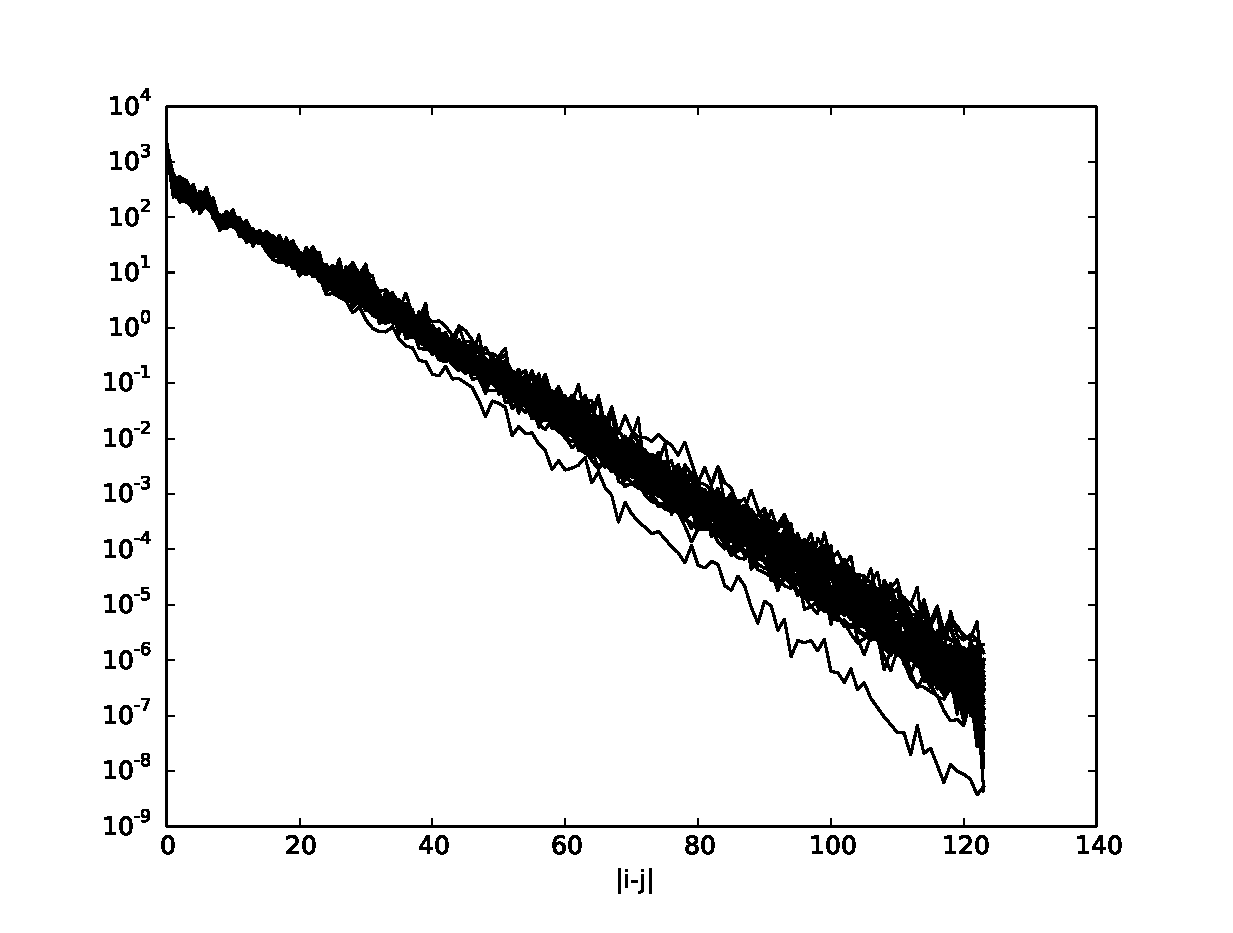
\includegraphics[width=1\linewidth]{./Figures/HessianDecayN30Tau1.eps}
  \caption{a) $\tau = 1$}
  \label{f:HessianDecayN30Tau1}
\end{subfigure}%
\begin{subfigure}{.5\linewidth}
  \centering
  \includegraphics[width=1\linewidth]{./Figures/HessianDecayN30Tau10minus6.eps}
  \caption{b) $\tau = 10^{-6}$}
  \label{f:HessianDecayN30Tau10minus6}
\end{subfigure}
\caption{Illustration of the off-diagonal decay. Each line corresponds to different $\lambda$.}
\label{fig:test}
\end{figure}

As discussed previously, the conditioning of $\Lambda_k$ affects the decaying property and small values of $\tau$ would therefore possibly lead to a slower decay. Corresponding figures to Figure \ref{f:HessianSpyN30Tau1} and Figure \ref{f:HessianDecayN30Tau1}, for $\tau = 10^{-6}$, are shown in Figure \ref{f:HessianSpyN30Tau10minus6} and Figure \ref{f:HessianDecayN30Tau10minus6} respectively. Observe that, for this example, there is no significant difference in the decay between the different values of $\tau$. This is also consistent with what we have observed in experiments with other problems.

The parameter, that according to our experiments, has the strongest impact on the decaying is the length of the horizon. To illustrate this, we generate another random problem with $N=10$, and all other dimensions being the same as before. The dual Hessian at the solution $\lambda^*(\tau)$, for $\tau=1$ is visualized in Figure \ref{f:HessianSpyN10Tau1}. Observe that the dual Hessian also in this case has a clear decay towards the off-diagonal corners. The band with elements of a significant magnitude is however wider compared to the size of the matrix. Moreover, the decaying property is visualized for $50$ different values of $\lambda$ in Figure \ref{f:HessianDecayN10Tau1}. Note that in this figure it is easier to see that there is a smaller difference between the diagonal and the off-diagonal elements.

\begin{figure}[h]
  \centering
  \includegraphics[scale=0.4]{./Figures/HessianSpyN10Tau1.eps}
  \caption{Illustration of the dual Hessian evaluated at $\lambda^*(\tau)$.}
  \label{f:HessianSpyN10Tau1}
\end{figure}

\begin{figure}[h]
  \centering
  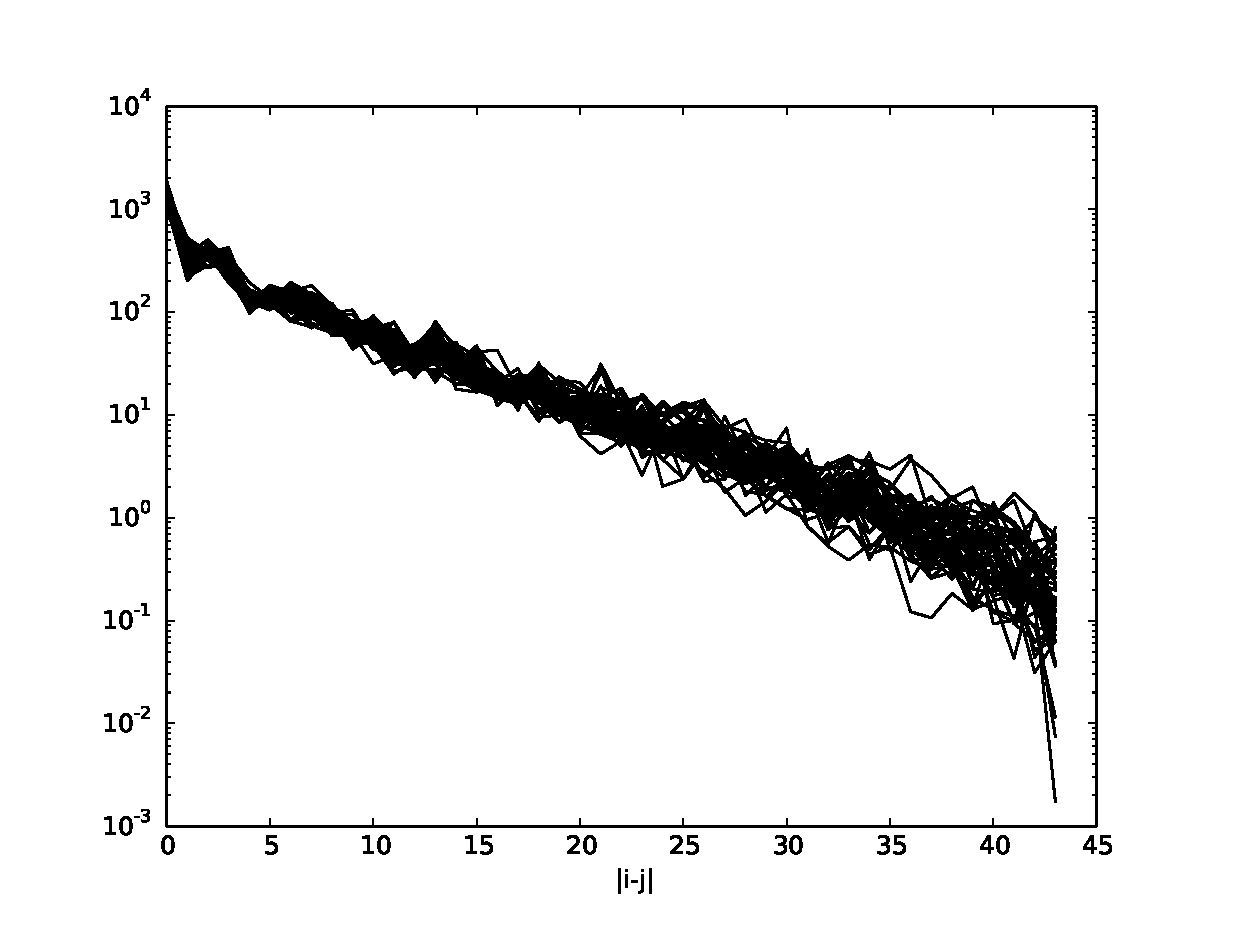
\includegraphics[scale=0.4]{./Figures/HessianDecayN10Tau1.eps}
  \caption{Illustration of the off-diagonal decay. Each line corresponds to different $\lambda$.}
  \label{f:HessianDecayN10Tau1}
\end{figure}


%\begin{acknowledgements}
%If you'd like to thank anyone, place your comments here
%and remove the percent signs.
%\end{acknowledgements}

% BibTeX users please use one of
%\bibliographystyle{spbasic}      % basic style, author-year citations
\bibliographystyle{spmpsci}      % mathematics and physical sciences
%\bibliographystyle{spphys}       % APS-like style for physics
%\bibliography{}   % name your BibTeX data base

% Non-BibTeX users please use
\bibliography{optec}

\end{document}
% end of file template.tex

